% !TeX program = xelatex
% !TeX encoding = UTF-8
\documentclass{MathorCupmodeling}
\let\kaishu\relax
\newCJKfontfamily\kaishu{KaiTi}[AutoFakeBold] %use fake KaiTi
\usepackage{zhlipsum,mwe}%use random characters
\usepackage{mathtools}%use mathtools
\usepackage{amsmath}
\usepackage{siunitx}
\usepackage{graphicx}
\usepackage{enumitem}
\setlist{nosep}

\begin{document}
\begin{center}
{\Large LQR}

\end{center}
    \newpage

%-------------------------------------------------------------------

	\section{$LQR$线性二次型调节器}

\subsection{$LQR$介绍}

LQR(linear quadratic regulator)线性二次型调节器,利用现代控制理论中以状态空间矩阵形式给出的线性系统,利用目标函数(能量函数)$J=\frac{1}{2}\int_0^\infty(x^TQx+u^TRu)dt$(其中Q为半正定矩阵,R为正定矩阵),设计状态反馈控制器$K$使得目标函数的值最小。
LQR控制器可以在系统偏离平衡状态时,尽可能减少消耗的能量保持系统状态各分量仍接近平衡状态.以一维系统$X=x(t)$为例,则$x^TQx=Qx^2$,为了使得$J$最小,那么该函数一定有界,故有下式

\begin{equation}
\lim_{t \rightarrow \infty}x(t)=0
\end{equation}

这保证了系统的稳定性,类似的$u(t)$小保证了节省能量,控制代价降低。

\subsection{$LQR$控制器原理性推导}

线性系统的状态空间可以描述为
	
\begin{equation}
\begin{aligned}
\dot X=AX+Bu\\
Y=CX+Du\\
\end{aligned}
\end{equation}

评价函数为

\begin{equation}
J=\frac{1}{2}\int_0^\infty(x^TQx+u^TRu)dt
\end{equation}

$Q、R$分别是对状态变量和输入量的加权矩阵,确定误差和能量损耗的相对性。

根据极小值原理,引入$n$维协态矢量$\lambda(t)$,构造哈密顿函数

\begin{equation}
H(x,u,\lambda)=\frac{1}{2}[x^TQx+u^TRu]+\lambda^T[Ax+Bu]
\end{equation}

最优控制使得$H$取极值,即

\begin{equation}
\frac{\partial H}{\partial u}=Ru+B^T\lambda=0
\end{equation}

解得

\begin{equation}
u=-R^{-1}B^T\lambda
\end{equation}

又有

\begin{equation}
\frac{\partial^2 H}{\partial u^2}=R
\end{equation}

R正定,故上式为系统的最优控制律。

设$\lambda=Px$,$P$为$n$阶实对称正定矩阵,且满足黎卡提矩阵代数方程

\begin{equation}
-PA-A^TP+PBR^{-1}B^T-Q_1=0
\end{equation}

则最优控制

\begin{equation}
u=-R^{-1}B^T\lambda=-Kx
\end{equation}

系统最优轨线为

\begin{equation}
\dot x(t)=(A-BK)x(t)
\end{equation}

在$matlab$中可以利用$lqr$函数求得反馈矩阵$K$.

\subsection{$LQR$的系统能控性和能观性分析}

对于上面假设的线性系统,状态完全能控制的充要条件是

\begin{equation}
rank[B,AB,A^2B,\dots A^{n-1}B]=n
\end{equation}

系统状态能够完全观测的充要条件是

\begin{equation}
rank
\begin{bmatrix}
C\\
CA\\
CA^2\\
\vdots\\
CA^{n-1}\\
\end{bmatrix}
=n
\end{equation}

\subsection{小车系统权重的选取以及能控性能观性分析}

前面得到小车的状态空间方程为

\begin{equation}
\begin{aligned}
&\begin{bmatrix}
\dot x\\
\ddot x\\
\dot{\varphi}\\
\ddot{\varphi}\\
\end{bmatrix}
=
\begin{bmatrix}
0 & 1 & 0 & 0\\
0 & 0 & 0 & 0\\
0 & 0 & 0 & 1\\
0 & 0 & 29.4 & 0\\
\end{bmatrix}
\begin{bmatrix}
x\\
\dot x\\
\varphi\\
\dot{\varphi}\\
\end{bmatrix}
+
\begin{bmatrix}
0\\
1\\
0\\
3\\
\end{bmatrix}
u'\\
&\begin{bmatrix}
x\\
\varphi\\
\end{bmatrix}
=
\begin{bmatrix}
1 &0 &0 &0\\
0 &0 &1 &0\\
\end{bmatrix}
\begin{bmatrix}
x\\
\dot x\\
\varphi\\
\dot{\varphi}\\
\end{bmatrix}
+
\begin{bmatrix}
0\\
0\\
\end{bmatrix}
u^{'}\\
\end{aligned}
\end{equation}

在$matlab$中(代码见附录)进行矩阵秩计算可知两个判定矩阵的秩都是$4$,则小车倒立摆系统可控可观测。

\subsection{小车倒立摆仿真}

首先根据系统的运动微分方程在$matlab$中的$simulink$进行仿真,由上述矩阵导出参考方程,为方便,将一些量名称更改如下

\begin{equation}
\begin{aligned}
&\dot x\rightarrow \dot x_1\\
&\ddot x\rightarrow \dot x_2\\
&\dot \varphi \rightarrow \dot x_3\\
&\ddot \varphi \rightarrow \dot x_4\\
\end{aligned}
\end{equation}

则有

\begin{equation}
\begin{aligned}
&\dot x_1=x_2\\
&\dot x_2=u\\
&\dot x_3=x_4\\
&\dot x_4=29.4x_3+3u\\
&u=-k_1x_1-k_2x_2-k_3x_3-k_4x_4\\
\end{aligned}
\end{equation}

得到如\cref{LQR_simulink}的仿真

\begin{figure}[hbpt]
\centering
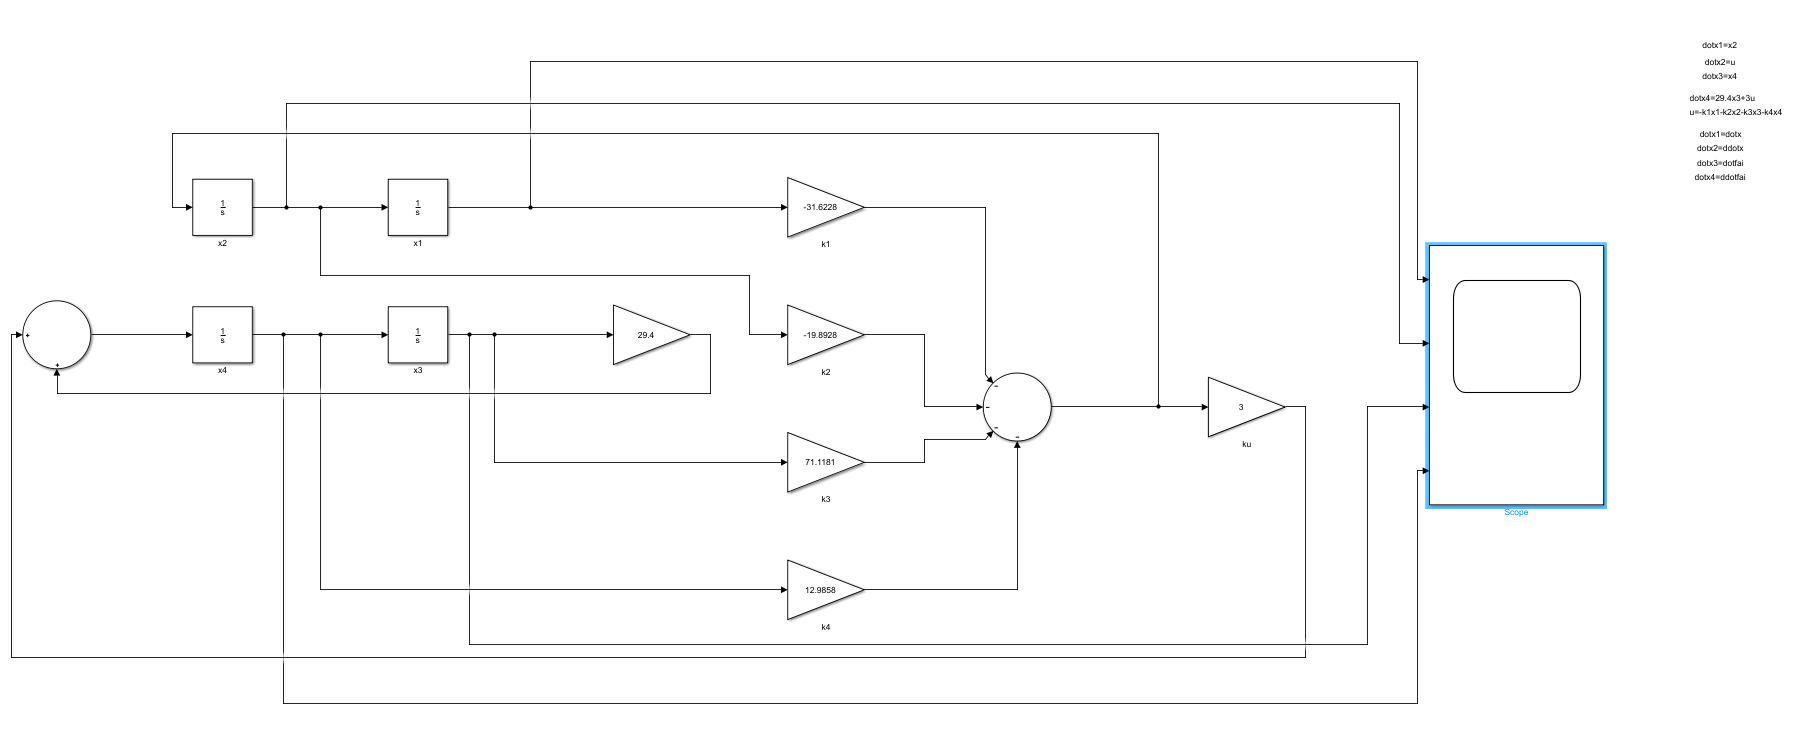
\includegraphics[width=16cm]{LQR_simulink.png}
\caption{$LQR的simulink$}\label{LQR_simulink}
\end{figure}

这种仿真可以通过给定$x_i$的初始值来模拟脉冲激励

\begin{figure}[hbpt]
\centering
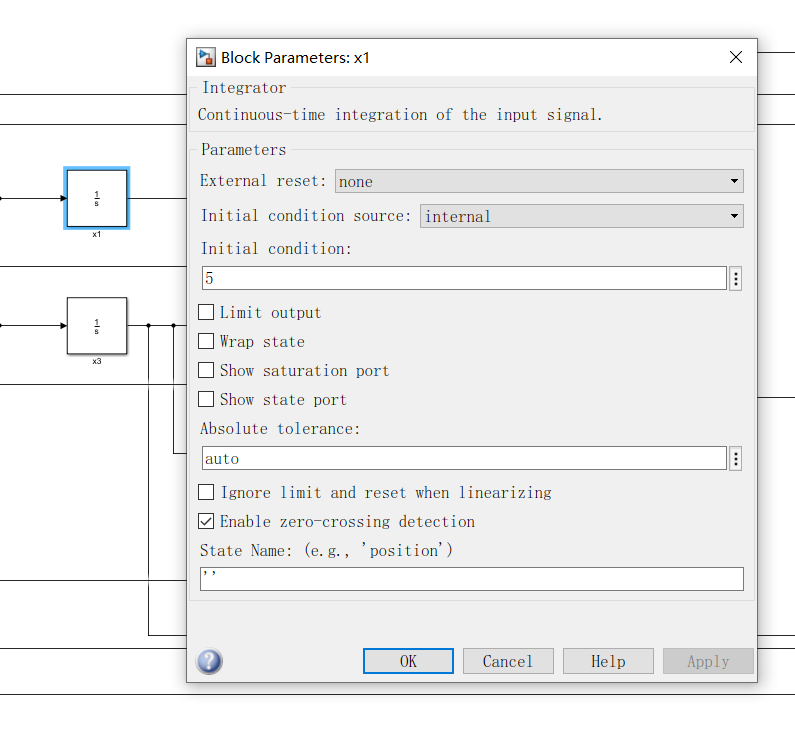
\includegraphics[width=12cm]{initial.png}
\caption{模拟脉冲激励}\label{initial}
\end{figure}

给定小车$5$单位位移,摆杆$5$单位角度,可以得到如\cref{1000_100}的响应曲线。

\begin{figure}[hbpt]
\centering
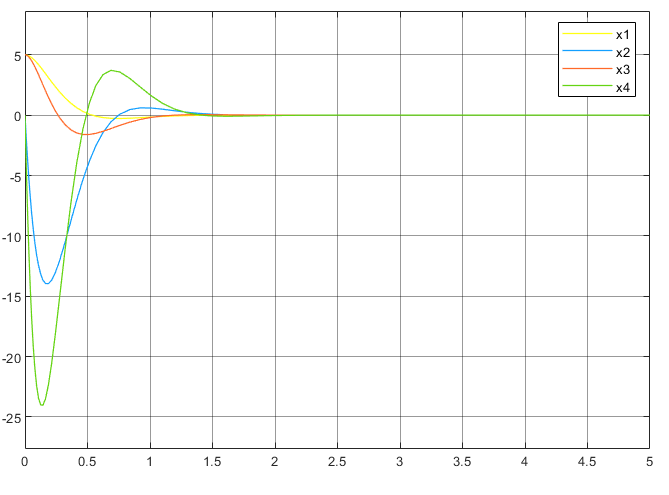
\includegraphics[width=12cm]{1000_100.png}
\caption{脉冲激励仿真结果}\label{1000_100}
\end{figure}

可以发现系统可以稳定。关于修改权重以及关于曲线的比较分析在后面介绍。

此外也可以利用编程来模拟仿真,以$lsim$函数模拟的阶跃信号为例,编写代码(见附件)也可以得到响应曲线如\cref{1000_100_2}

\begin{figure}[hbpt]
\centering
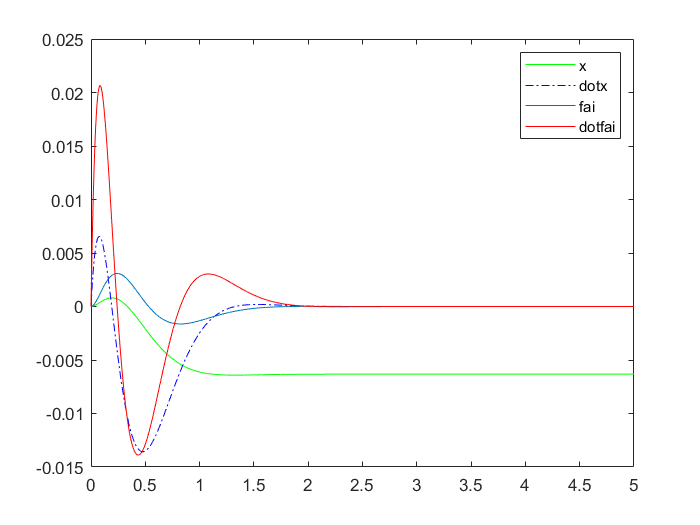
\includegraphics[width=12cm]{1000_100_2.png}
\caption{阶跃激励仿真结果}\label{1000_100_2}
\end{figure}

\subsection{修改权重分析比较}

依次修改$Q_{11}Q_{22}Q_{33}Q_{44}$权重(值见图片),建立如\cref{比较仿真}的仿真

\begin{figure}[hbpt]
\centering
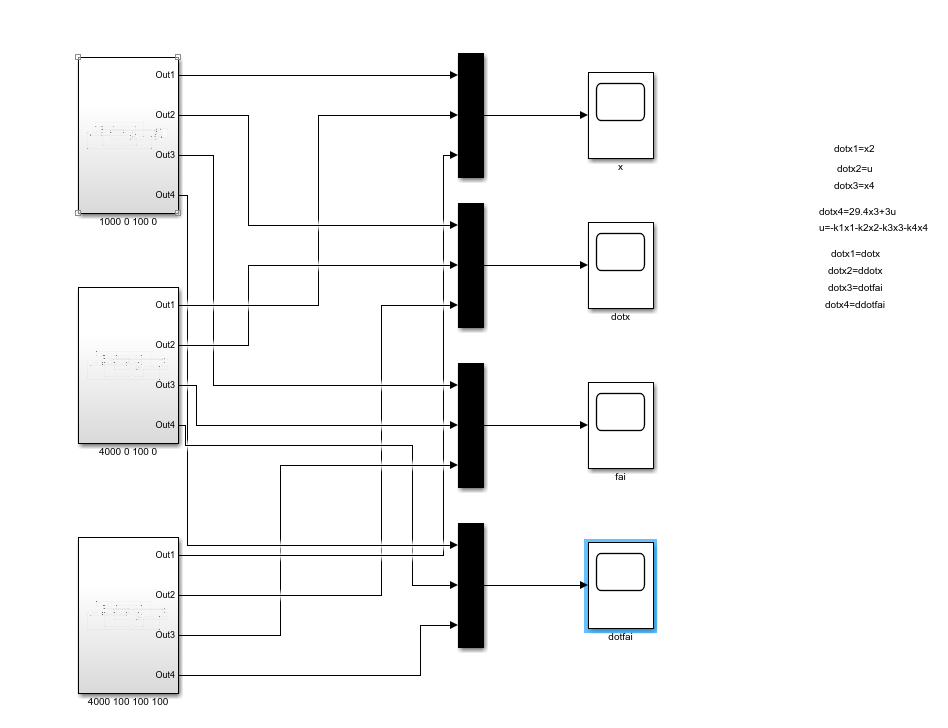
\includegraphics[width=12cm]{比较仿真.png}
\caption{比较仿真}\label{比较仿真}
\end{figure}

观察比较仿真结果如\cref{数据比较}
\begin{figure}[hbpt]
\centering
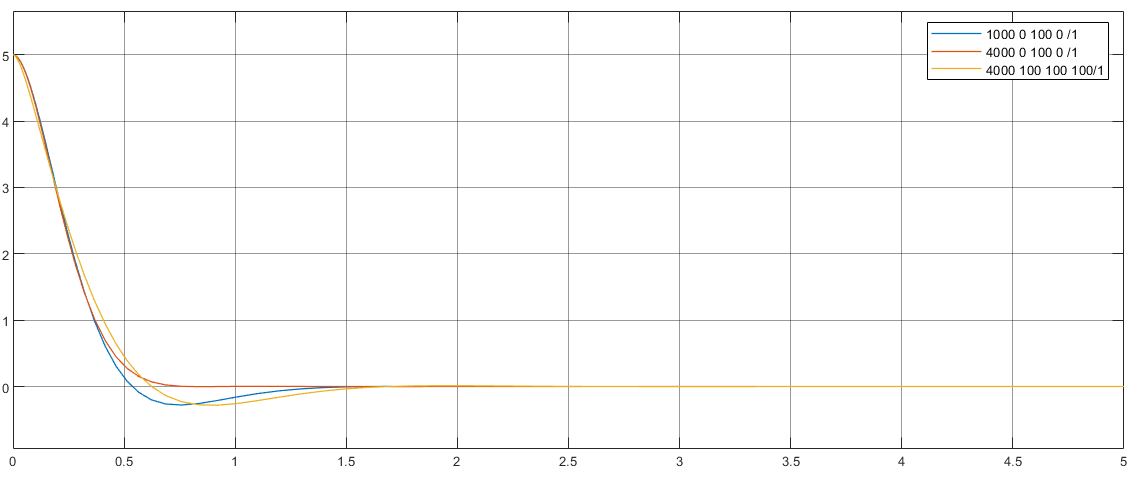
\includegraphics[width=12cm]{x.png}
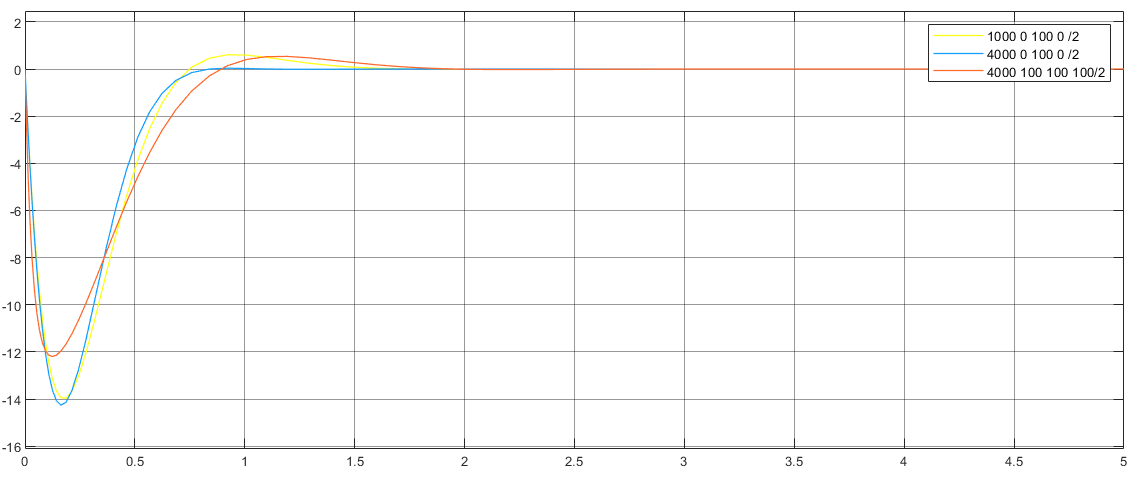
\includegraphics[width=12cm]{dotx.png}
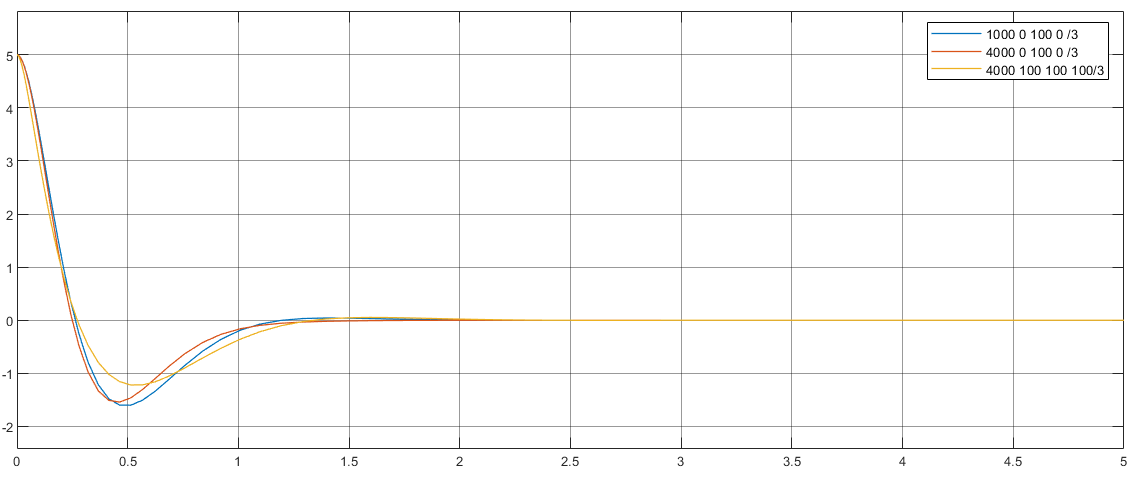
\includegraphics[width=12cm]{fai.png}
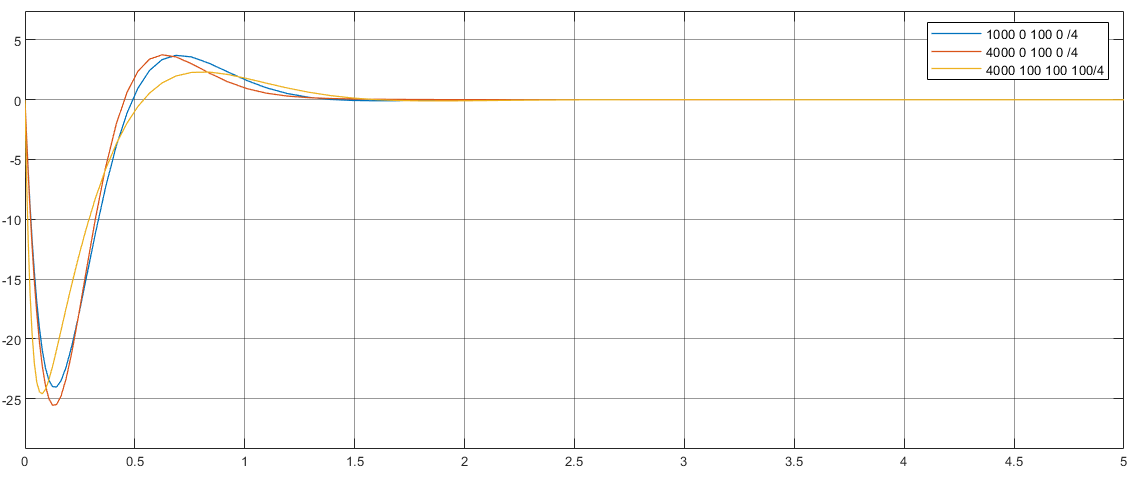
\includegraphics[width=12cm]{dotfai.png}
\caption{数据比较}\label{数据比较}
\end{figure}

不难发现这三组数据都可以保证小车和摆杆的稳定性,都可以比较快速的达到稳定状态,区别就是随着权重的增大,控制目标变量可以更快的达到稳定,并且超调量变小,但是权重的变大意味着输入的能耗增加(如\cref{u}),不是最经济的选择.

\begin{figure}[hbpt]
\centering
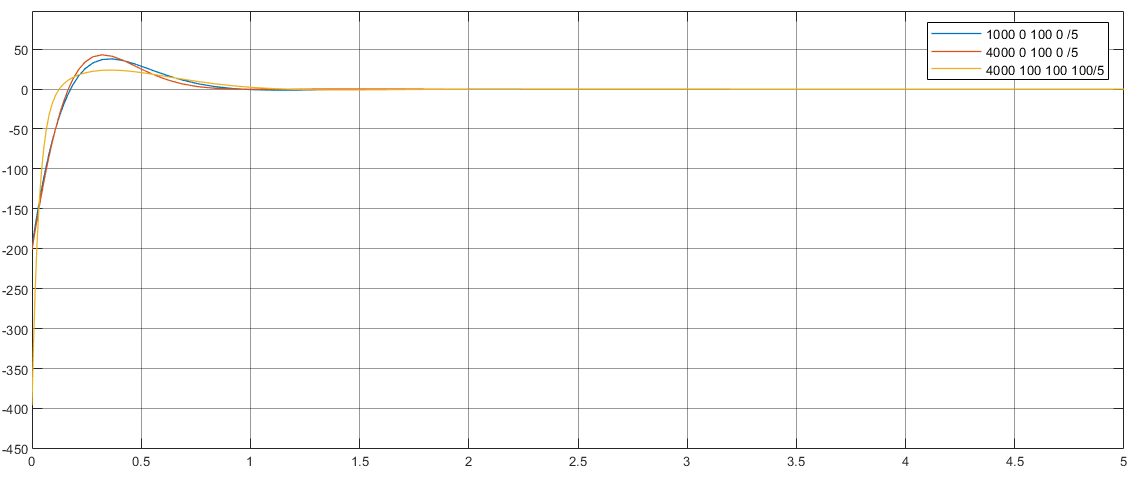
\includegraphics[width=12cm]{u.png}
\caption{u}\label{u}
\end{figure}

因此,在可以快速的稳定这个前提下,应该尽可能减小权重值。最终我们选定$Q11=1000,Q33=100$这个权重值,其对应$K$矩阵为

\begin{equation}
K=
\begin{bmatrix}
-31.6228\\
-19.8928\\
-71.1181\\
12.9858\\
\end{bmatrix}
\end{equation}
\newpage
%-----------------------------------------------------
	\appendix
	\ctexset{section={
		format={\zihao{-4}\heiti\raggedright}
	}}
	\begin{center}
		\heiti\zihao{4} 附\hspace{1pc}录
	\end{center}

\begin{matlab}
%系统能控性与能观性判定
A=[0 1 0 0;
   0 0 0 0;
   0 0 0 1;
   0 0 29.4 0];
B=[0 1 0 3]';
C=[1 0 0 0;
   0 0 0 1];
D=[0 0]';
Co=ctrb(A,B);
rank(Co)
Ob=obsv(A,C);
rank(Ob)
\end{matlab}

\begin{matlab}
%模拟阶跃信号 
A=[0 1 0 0;0 0 0 0;0 0 0 1;0 0 29.4 0];
B=[0 1 0 3]';
C=[1 0 0 0;0 0 1 0];
D=[0 0 ]';
Q11=1000;
Q33=100;%该值可以更改
Q=[Q11 0 0 0;0 0 0 0;0 0 Q33 0;0 0 0 0];
R=1;
K=lqr(A,B,Q,R);
Ac=(A-B*K);
T=0:0.001:5;
U=0.2*ones(size(T));
[Y,X]=lsim(Ac,B,C,D,U,T);%模拟阶跃输入
plot(T,X(:,1),'-g','LineWidth',1);
hold on;
plot(T,X(:,2),'-.b','LineWidth',1);
plot(T,X(:,3),'-','LineWidth',1);
plot(T,X(:,4),'-r','LineWidth',1);
hold off;
legend('x','dotx','fai','dotfai');
\end{matlab}


\end{document}